% !TeX spellcheck = ru_RU
% !TeX encoding = UTF-8
\subsection{Защитный интервал}
В английской литературе зущитный интервал --- Guard Interval.
Важно сразу отметить, существуют различные техники для борьбы с помехами при передаче по радио 
каналу. В данном разделе будет рассмотрен <<Защитный интервал>>, как средство для борьбы со взаимной
интерфифренцией сигнала рисунок~\ref{fig:kov_interf}, возникающей в следствие наличия замираний в канале.

Если путь от передатчика к приемнику имеет отражения или 
препятствия, либо и то и другое, мы можем получить эффект замирания. В этом случае, сигнал достигает
приемника разными путями, каждый из которых --- копия оригинала. Каждый из этих лучей имеет
немного разную задержку и немного разное усиление. Временные задержки выливаются в
фазовые сдвиги, которые накладываются на компоненту основного сигнала (если таковой
имеется), вызывая ухудшение сигнала.

\begin{figure}[H]
    \centering
    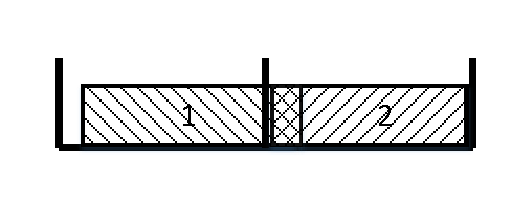
\includegraphics[width=0.5\textwidth]{img/kov_interf}
    \caption{Интерференция двух сообщений}
    \label{fig:kov_interf}
\end{figure}

Защитным интервалом называют дополнение к сообщению, передаваемому по каналу, куда вставляется
циклический префикс (ЦП), где ЦП --- копия конца сообщения~\ref{fig:kov_CP} .

\begin{figure}[H]
    \centering
    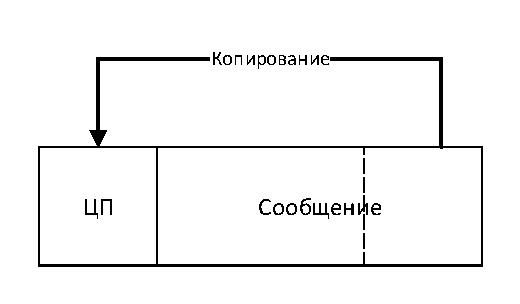
\includegraphics[width=0.5\textwidth]{img/kov_CP}
    \caption{Циклический префикс}
    \label{fig:kov_CP}
\end{figure}

Таким образом, если часть сообщения будет нарушена, как на рисунке~\ref{fig:kov_interf}, полезная 
информация не будет потеряна, так как дубликат хранится в ЦП, что позволяет полностью восстановить
сообщение на приёмной стороне, даже при наличии взаимной интерфиренции между сообщениями.